\documentclass{beamer}

\setbeamertemplate{background canvas}[vertical shading][bottom=cyan!10,top=blue!10]

\usetheme{Warsaw}
\usefonttheme[onlysmall]{structurebold}

% pour le fichiers .pdf
\usepackage{graphicx}
\usepackage{color}
% pour les fichiers .png
% \usepackage{pgf,pgfarrows}
% \usepackage{pgf,pgfarrows}
\usepackage{amsmath,amssymb}
\usepackage{textcomp}
\setbeamercovered{dynamic}
\DeclareMathOperator*{\argmin}{argmin}

\title[OpenTURNS developers training: agenda]{OpenTURNS developers training: agenda}
\author[OpenTURNS Consortium, 2019]
{
  Trainer : R\'egis LEBRUN\\ 
  Airbus \\
  regis.lebrun@airbus.com
}



\date[March 22-25th 2011]
{
  Developers training \\

  \begin{center}
    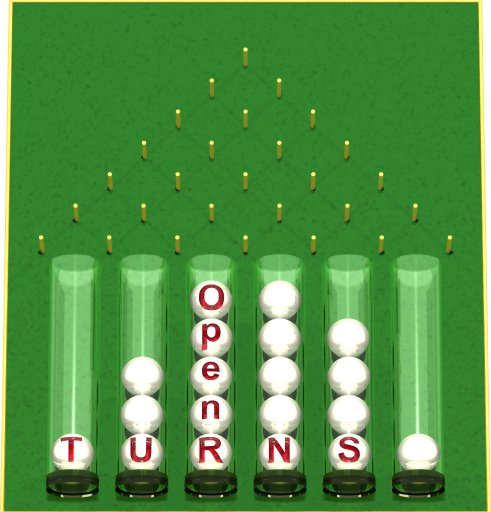
\includegraphics[height=2cm]{logoOT.jpg}
  \end{center}
}

\subject{OpenTURNS Developers Training}

% \part<presentation>{Corps de presentation}


\begin{document}

\frame{\titlepage}

% necessaire pour la table des matieres
\part{Main part}

%%%%%%%%%%%%%%%%%%%%%%%%%%%%% 
% Objective of the training %
%%%%%%%%%%%%%%%%%%%%%%%%%%%%% 
\begin{frame}
  \frametitle{The developers training}
  \begin{block}{Objectives}
    This 4 days training will give you the first elements to:
    \begin{itemize}
    \item Understand the OpenTURNS aim and architecture,
    \item Discover the coding rules, the development process and the associated infrastructure,
    \item Make your first steps in the OpenTURNS development by adding a new specialization of an existing concept both in the C++ library and the Python interface,
    \item Make your first steps in the OpenTURNS module development.
    \end{itemize}
  \end{block}
\end{frame}
%%%%%%%%%%%%%%%%%%%%%%%% 
% General organization %
%%%%%%%%%%%%%%%%%%%%%%%% 
\begin{frame}
  \frametitle{General organization}
  \begin{block}{Agenda}
    Each of these four days will be organized as follow:
    \begin{description}
    \item[9.30am] Welcome (coffee \& tea)
    \item[9.45am] Theory
    \item[12.15pm] Lunch
    \item[13.15pm] Theory or experimentation
    \item[15.15pm] Break (coffee \& tea)
    \item[15.30pm] Experimentation
    \item[17.30pm] End of the day
    \end{description}
  \end{block}
\end{frame}
%%%%%%%%%%%%%%%%%%%%%%%%%%%%%%%%%%%%%%%%%%%%%%% 
% Day 1: uncertainties, package, architecture %
%%%%%%%%%%%%%%%%%%%%%%%%%%%%%%%%%%%%%%%%%%%%%%% 
\begin{frame}
  \frametitle{Day by day...}
  \begin{block}{Day 1: uncertainties, OpenTURNS platform, architecture}
    \begin{itemize}
    \item Uncertainties: quick reminder on analysis, probability and statistics
    \item OpenTURNS platform: the global picture of OpenTURNS product and the website, short presentation of the development life-cycle.
    \item Architecture: the general organization of the product with some highlights on the key mechanisms and their implementation.
    \item Experimentation: basic manipulation of a numerical function and a probability distribution, navigation in the website (tickets, versioning system), exploration of examples in C++ and python.
    \item Selection of the challenges.
    \end{itemize}
  \end{block}
\end{frame}
%%%%%%%%%%%%%%%%%%%%%%%%%%%%%%%%%%%%%%%%%%%%%%%%%%%%%%%%% 
% Day 2: development in OpenTURNS: the C++ library part %
%%%%%%%%%%%%%%%%%%%%%%%%%%%%%%%%%%%%%%%%%%%%%%%%%%%%%%%%% 
\begin{frame}
  \frametitle{Day by day...}
  \begin{block}{Day 2: development in the C++ library}
    \begin{itemize}
    \item The development infrastructure: some elements on CMake.
    \item The development process: architecture, C++ implementation, tests.
    \item Experimentation: C++ implementation of the challenge.
    \end{itemize}
  \end{block}
\end{frame}
%%%%%%%%%%%%%%%%%%%%%%%%%%%%%%%%%%%%%%%%%%%%%%%%%%%% 
% Day 3: development in OpenTURNS: the python part %
%%%%%%%%%%%%%%%%%%%%%%%%%%%%%%%%%%%%%%%%%%%%%%%%%%%% 
\begin{frame}
  \frametitle{Day by day...}
  \begin{block}{Day 3: make the development visible in python}
    \begin{itemize}
    \item Interfacing C++ and Python using SWIG.
    \item The development process: SWIG interface, python modules, tests, documentation.
    \item Experimentation: Python binding and documentation of the challenge.
    \end{itemize}
  \end{block}
\end{frame}
%%%%%%%%%%%%%%%%%%%%%%%%%%%%%%%%%%%%%%%%%%%%%%%%%%%%%%%% 
% Day 4: development around OpenTURNS: create a module %
%%%%%%%%%%%%%%%%%%%%%%%%%%%%%%%%%%%%%%%%%%%%%%%%%%%%%%%% 
\begin{frame}
  \frametitle{Day by day...}
  \begin{block}{Day 4: create an OpenTURNS module}
    \begin{itemize}
    \item The concept of module, its standard structure.
    \item The key steps in the development of a module.
    \item How to install and use a module?
    \item Experimentation: implementation of the second challenge as a module.
    \end{itemize}
  \end{block}
\end{frame}
%%%%%%%%%%%%%% 
% Conclusion %
%%%%%%%%%%%%%% 
\begin{frame}
  \frametitle{Already a contributor}
  \begin{block}{You are a new OpenTURNS developer!}
    \begin{itemize}
    \item All the developments made during this training session will become part of OpenTURNS sooner or later, depending on their degree of maturity (quality ;) ?).
    \item The missing steps for a direct integration will be the testing phase, the validation phase and probably parts of the documentation phase.
    \item The integration will be done using a development branch on GitHub.
    \end{itemize}
    Check the upcoming release or the next to see your work in action!
  \end{block}
\end{frame}
\end{document}
